
\begin{figure}[H]
\centering
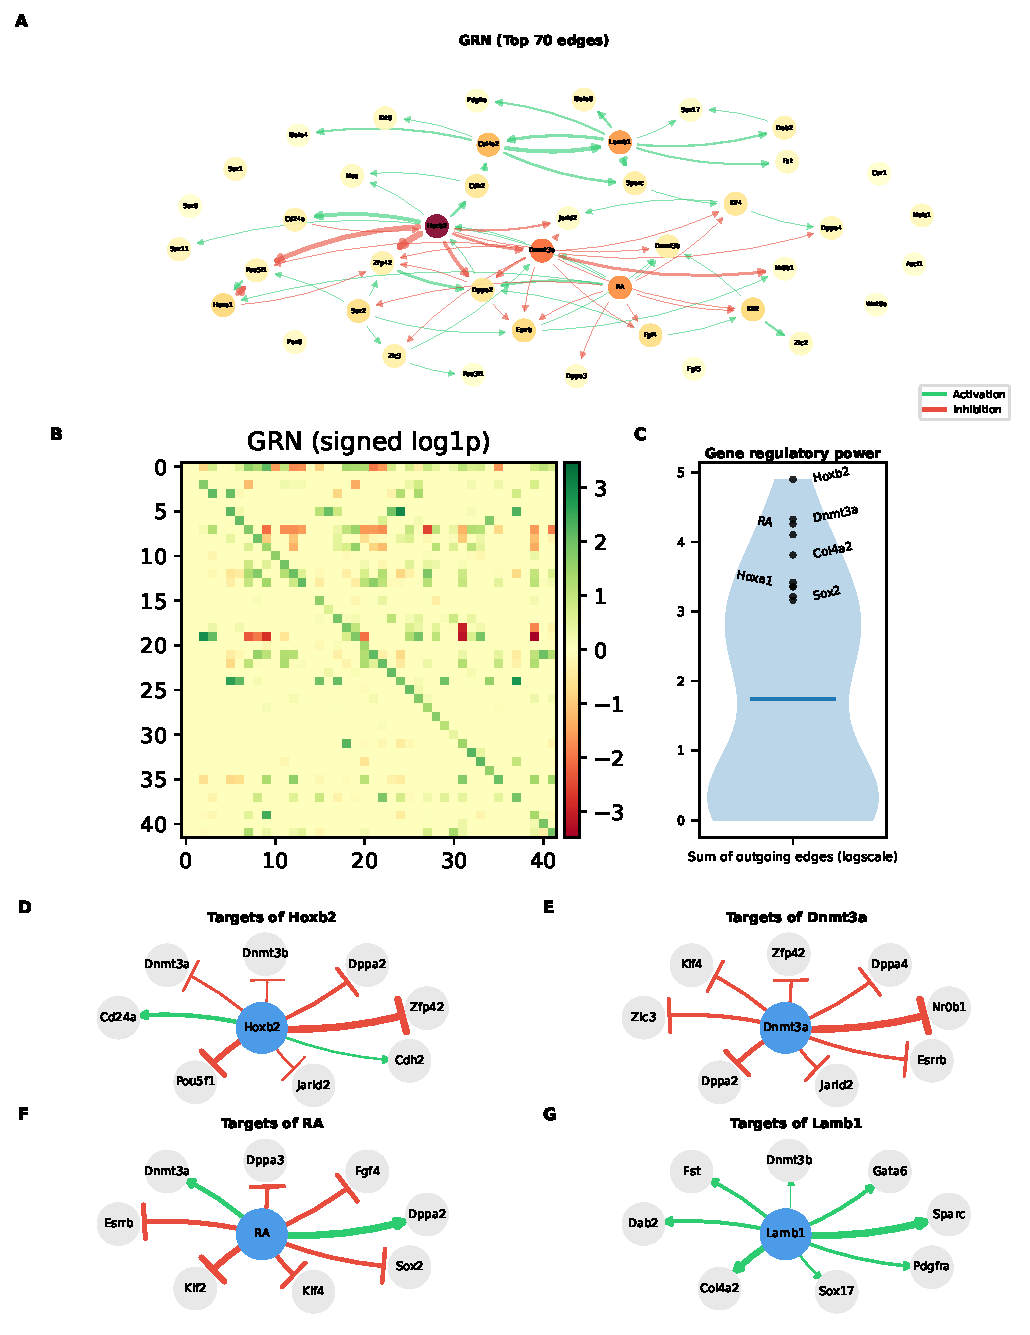
\includegraphics[width=\textwidth]{figureS1.pdf}
    \caption{Representation of the inferred gene regulatory network for the Semrau dataset. (A) Graph showing the top 70 edges of the GRN by absolute regulation strength, limited to a max of 5 incoming regulating edges for visualization. (B) Signed log1p transformed full GRN matrix representing the strength of all genes on each other, with lines being regulators and columns being targets. (C) Violin plot of dataset genes ranked by the sum of all their outgoing edges, with the top genes labeled. (D–G) Small GRN representation of the top regulators Hoxb2, Dnmt3a, RA and Lamb1, showing their top 8 regulatory targets.}
    \label{figure_S1}
\end{figure}

\begin{figure}[H]
\centering
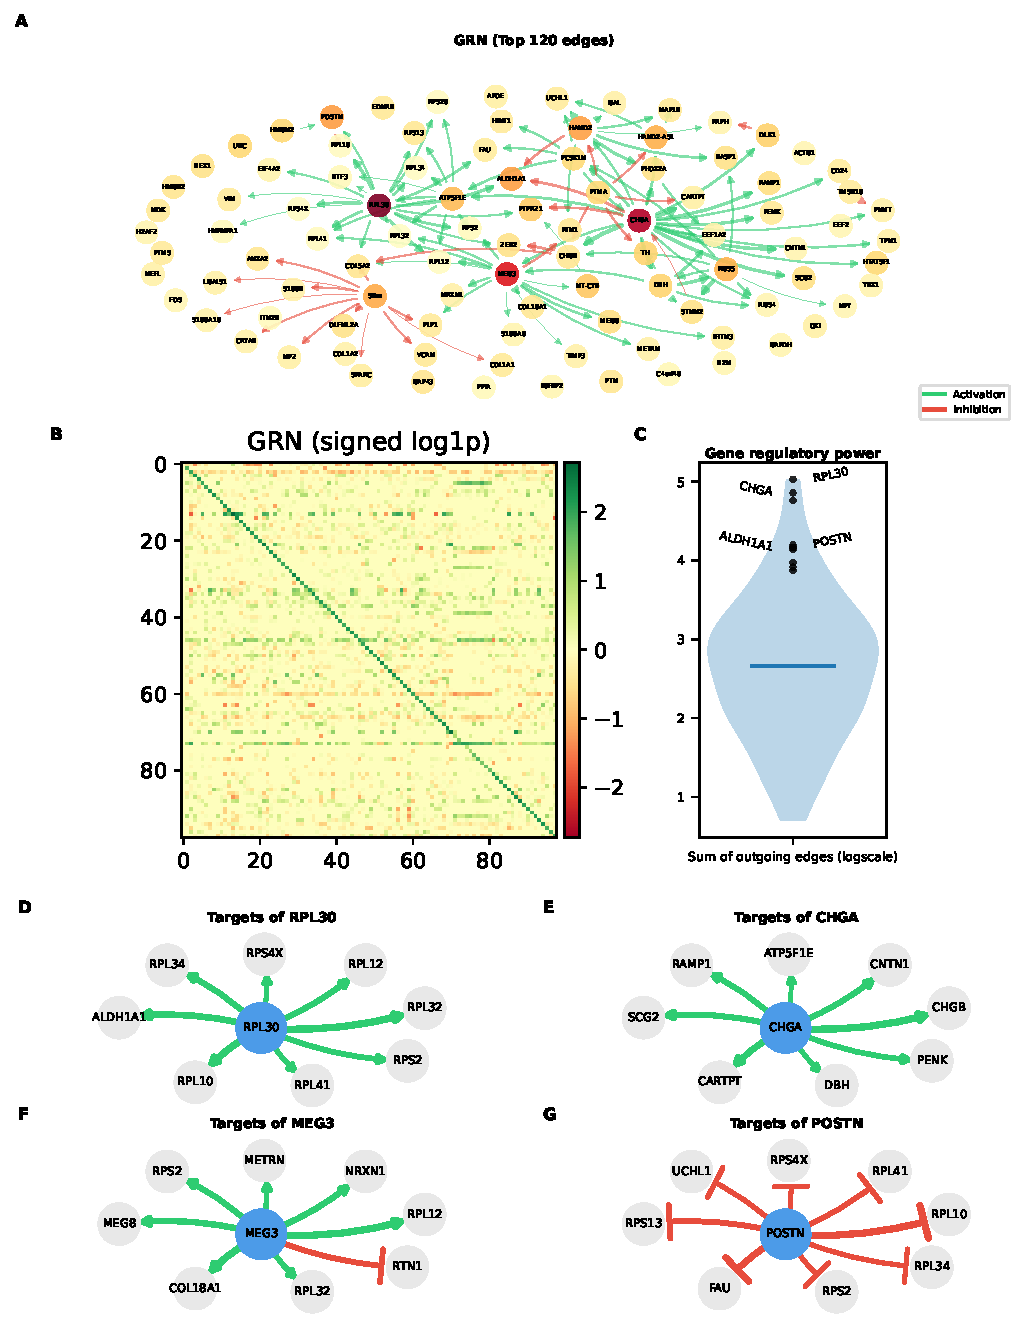
\includegraphics[width=\textwidth]{figureS2.pdf}
    \caption{Representation of the inferred gene regulatory network for the Kameneva dataset. (A) Graph showing the top 120 edges of the GRN by absolute regulation strength, limited to a max of 5 incoming regulating edges for visualization. (B) Signed log1p transformed full GRN matrix representing the strength of all genes on each other, with lines being regulators and columns being targets. (C) Violin plot of dataset genes ranked by the sum of all their outgoing edges, with the top genes labeled. (D–G) Small GRN representation of the top regulators RPL30, CHGA, MEG3 and POSTN, showing their top 8 regulatory targets.}
    \label{figure_S2}
\end{figure}

\begin{figure}[H]
\centering
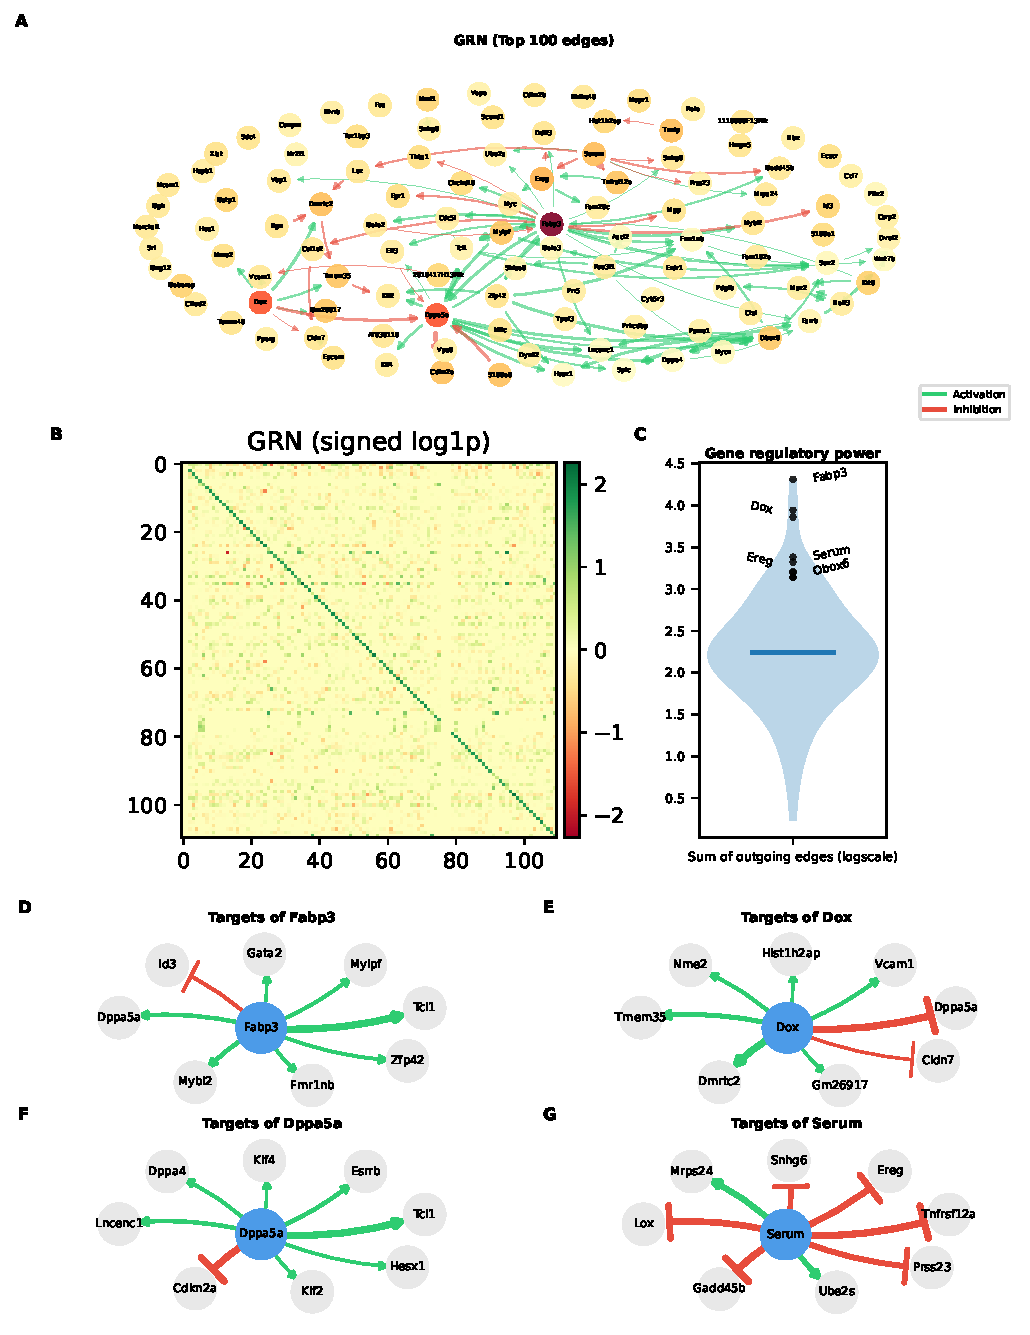
\includegraphics[width=\textwidth]{figureS3.pdf}
    \caption{Representation of the inferred gene regulatory network for the Schiebinger dataset. (A) Graph showing the top 100 edges of the GRN by absolute regulation strength, limited to a max of 5 incoming regulating edges for visualization. (B) Signed log1p transformed full GRN matrix representing the strength of all genes on each other, with lines being regulators and columns being targets. (C) Violin plot of dataset genes ranked by the sum of all their outgoing edges, with the top genes labeled. (D–G) Small GRN representation of the top regulators Fabp3 and Dppa5a, and of the two stimulus nodes Dox and Serum, showing their top 8 regulatory targets.}
    \label{figure_S3}
\end{figure}


\begin{figure}[H]
\centering
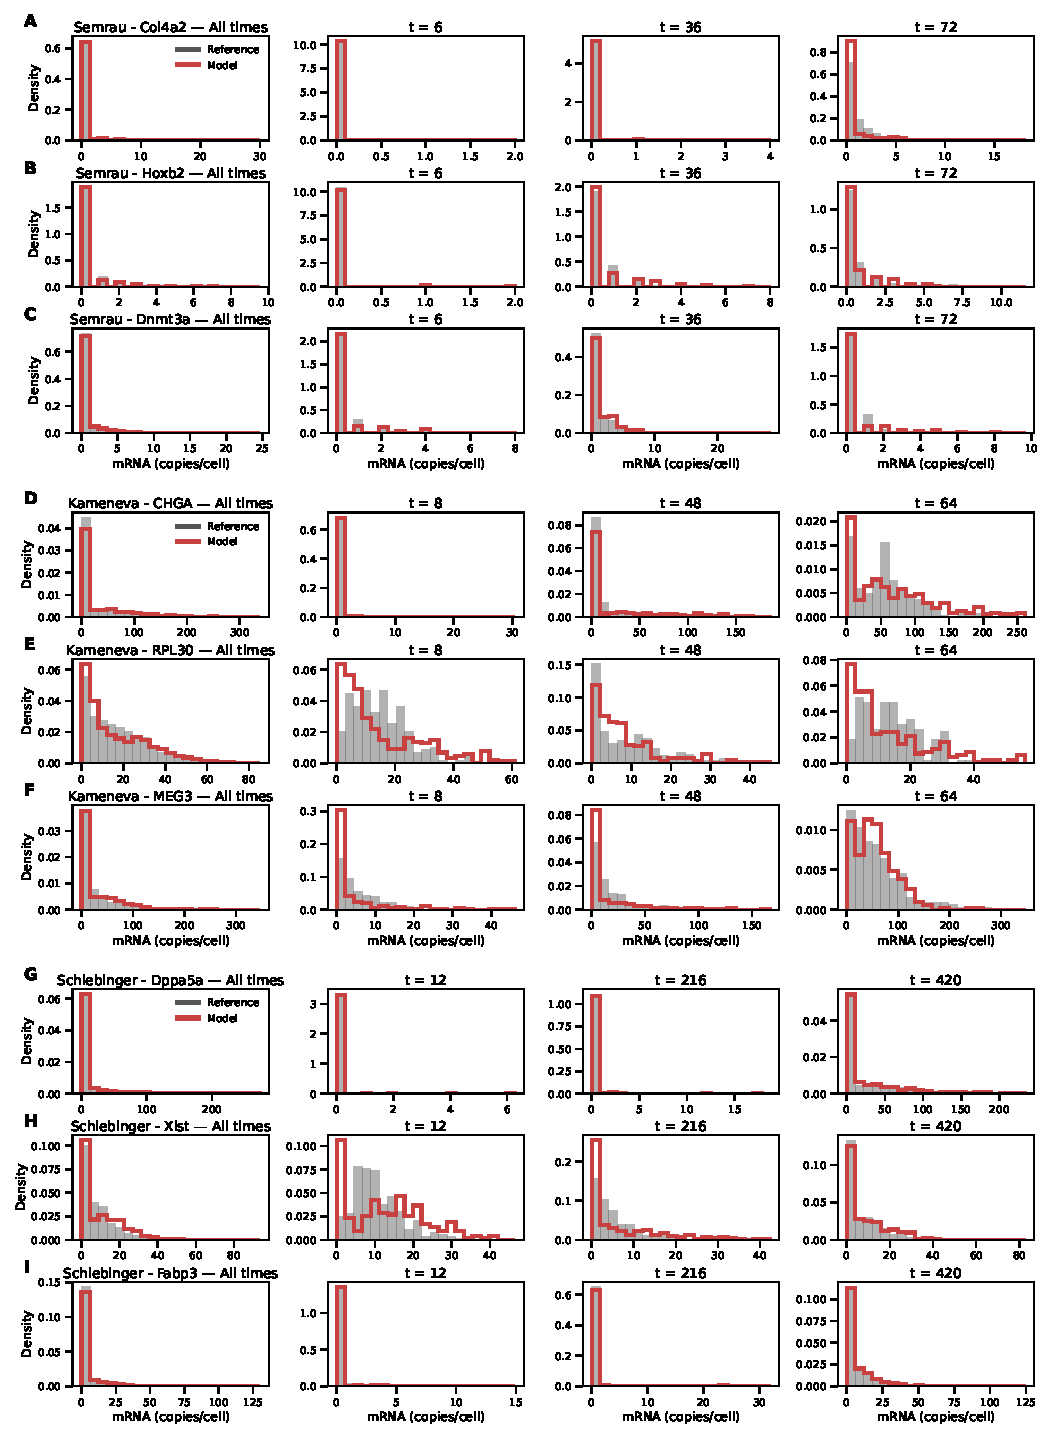
\includegraphics[width=\textwidth]{figureS4.pdf}
    \caption{Marginal mRNA distributions for selected genes, showing (leftmost column) 
    all timepoints joined and (remaining columns) three selected timepoints for each 
    gene. Three of the main regulators were selected for the Semrau (A--C), Kameneva 
    (D--F) and Schiebinger (G--I) datasets, namely \textit{Col4a2}, \textit{Hoxb2} and \textit{Dnmt3a} for 
    Semrau, \textit{CHGA}, \textit{RPL30} and \textit{MEG3} for Kameneva, and \textit{Dppa5a}, \textit{Xist} and \textit{Fabp3} for 
    Schiebinger. Marginal distributions are shown for the reference data (gray) and 
    the Negative Binomial mixture model (red).}
    \label{figure_S4}
\end{figure}


\begin{figure}[H]
\centering
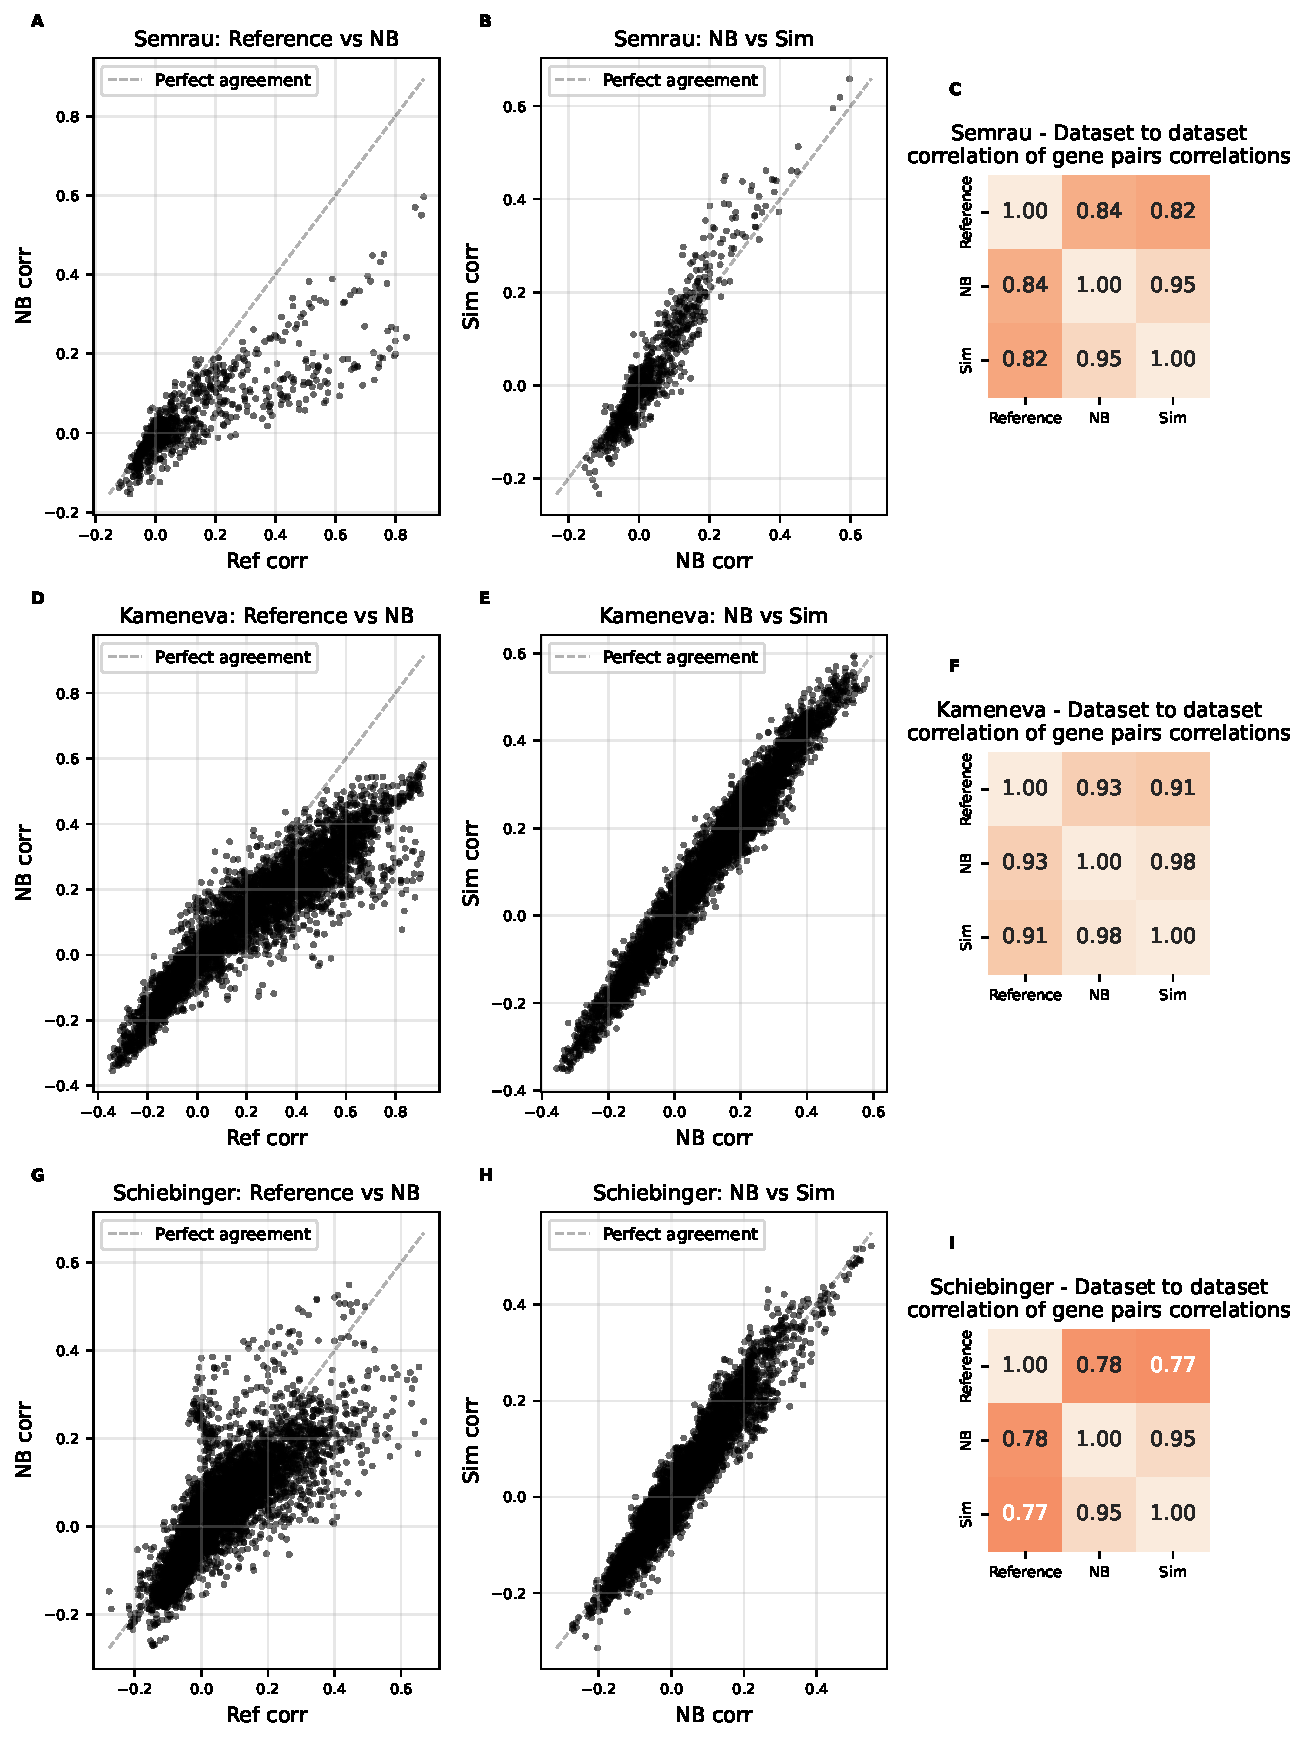
\includegraphics[width=.9\textwidth]{figureS5.pdf}
    \caption{Pairwise gene expression correlation structure across reference, NB mixture 
    and simulated datasets, for the Semrau (A--C), Kameneva (D--F) and Schiebinger 
    (G--I) datasets. (A, D, G) Scatter plots of pairwise gene correlations computed 
    from the reference data versus those computed from the NB mixture model, with the 
    dashed line indicating perfect agreement. (B, E, H) Same comparison between the NB 
    mixture model and the full generative model simulations. (C, F, I) Dataset-to-dataset 
    correlation matrices summarizing the Pearson correlation between the vectors of all 
    pairwise gene correlations across the three datasets (Reference, NB, Sim), providing 
    a global measure of how well each model reproduces the correlation structure of the 
    reference data.}
    \label{figure_S5}
\end{figure}


\begin{figure}[H]
\centering
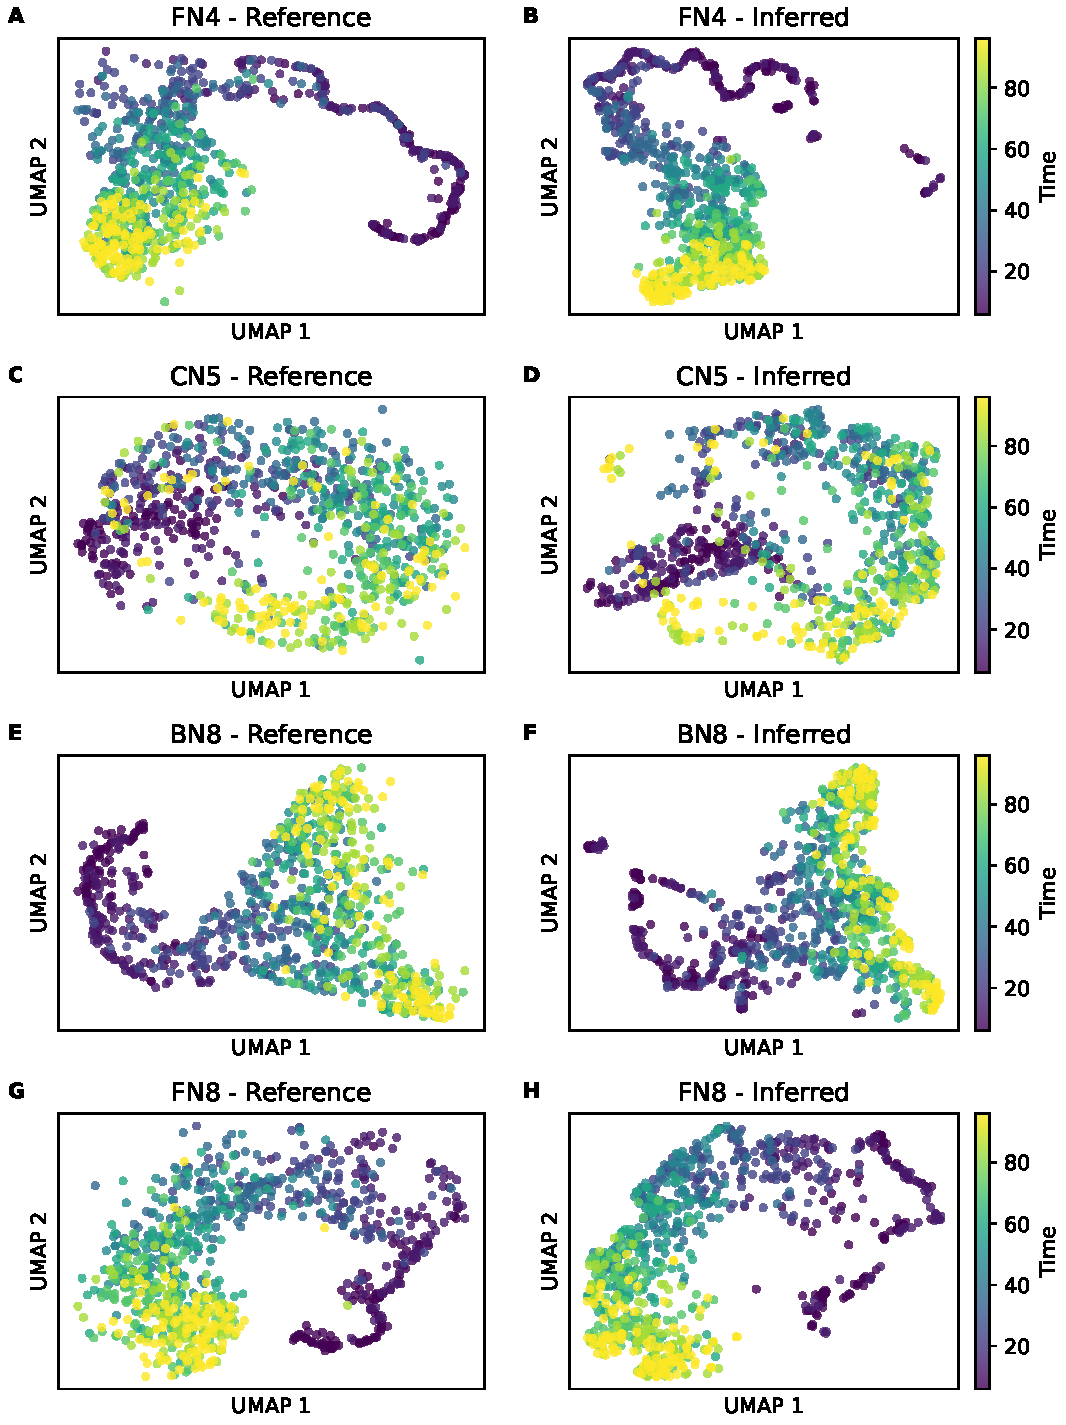
\includegraphics[width=\textwidth]{figureS6.pdf}
    \caption{UMAPs of reference and CardamomOT inferred protein trajectories for the 
    (A--B) FN4, (C--D) CN5, (E--F) BN8 and (G--H) FN8 datasets. (A, C, E, G) UMAPs 
    of reference simulated protein trajectories are reproduced by (B, D, F, H) inferred 
    protein trajectories from the reference protein-associated RNA data.}
    \label{figure_S6}
\end{figure}


\begin{figure}[H]
\centering
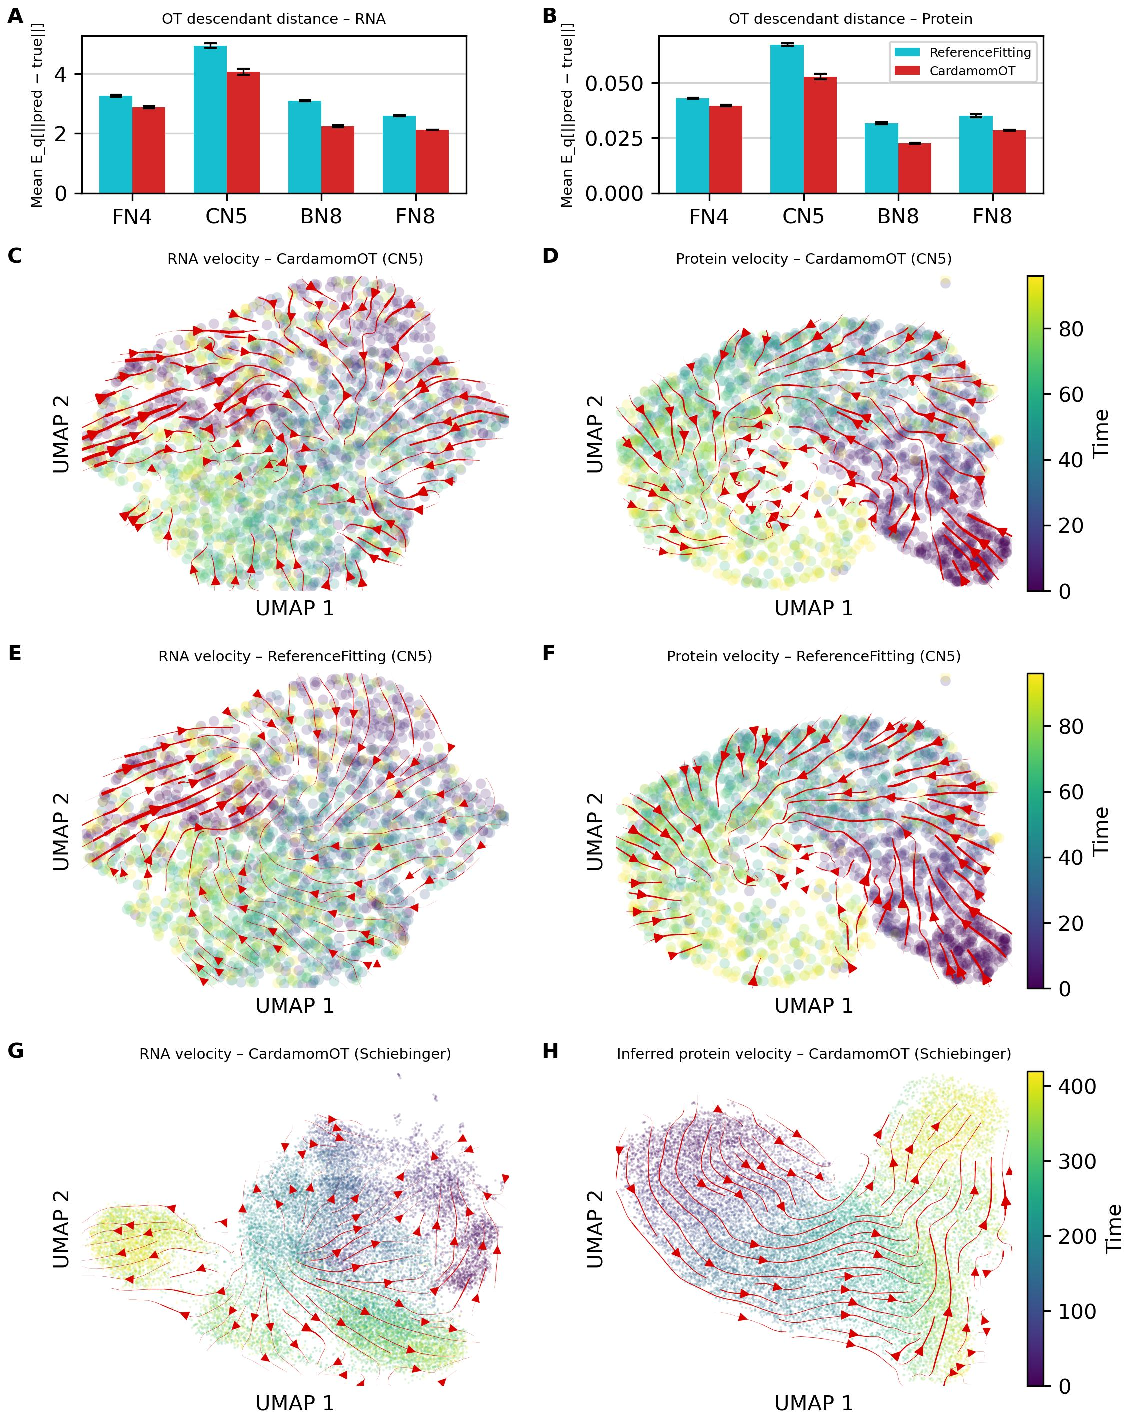
\includegraphics[width=\textwidth]{figureS7.pdf}
    \caption{Evaluation of the cell-to-cell coupling accuracy on true 
    trajectory data for CardamomOT and Reference Fitting. (A--B) OT descendant distance for mRNA (A) and protein (B): Bars show the mean over 5 
    independent simulations of true trajectories per network; error bars indicate the standard 
    error. (C--F) UMAP embeddings of RNA (C,E) and protein (D,F) expression of CN5 benchmark 
    cells simulated as true trajectories, with velocity stream plots derived from the inferred 
    couplings of CardamomOT (C--D) and Reference Fitting (E--F). (G--H) UMAP of RNA (G) 
    and inferred protein (H) data from Schiebinger et al.\ 2019 \cite{schiebinger2019optimal}, 
    with CardamomOT velocity stream plots derived from the inferred trajectories.}
    \label{figure_S7}
\end{figure}


\begin{figure}[H]
  \centering
  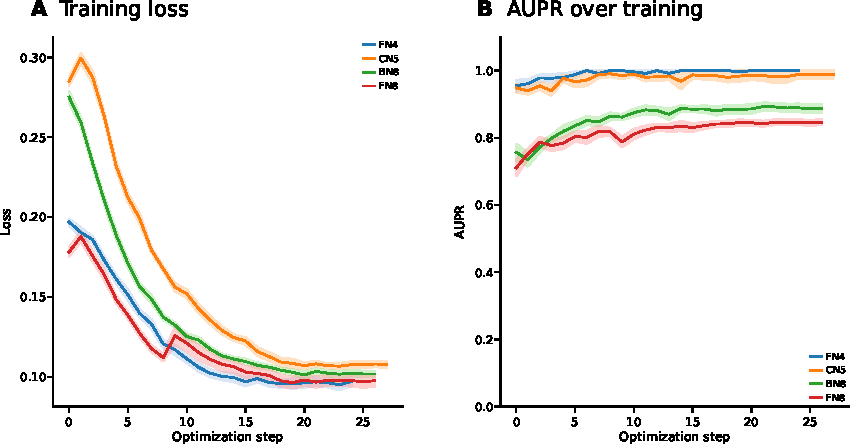
\includegraphics[width=0.9\textwidth]{figureS8.pdf}%
  \caption{%
Evolution of the loss function and AUPR score during training for the networks FN4, CN5, BN8, and FN8 used in the Benchmark of Figures \ref{figure3} and \ref{figure4}. (A) Mean training loss at each optimization step, averaged over 10 independent runs, with shaded bands indicating the uncertainty (standard error). (B) The corresponding evolution of the AUPR score over the same training steps and networks.%
}
  \label{figure_S8}
\end{figure}


\begin{figure}[H]
  \centering
  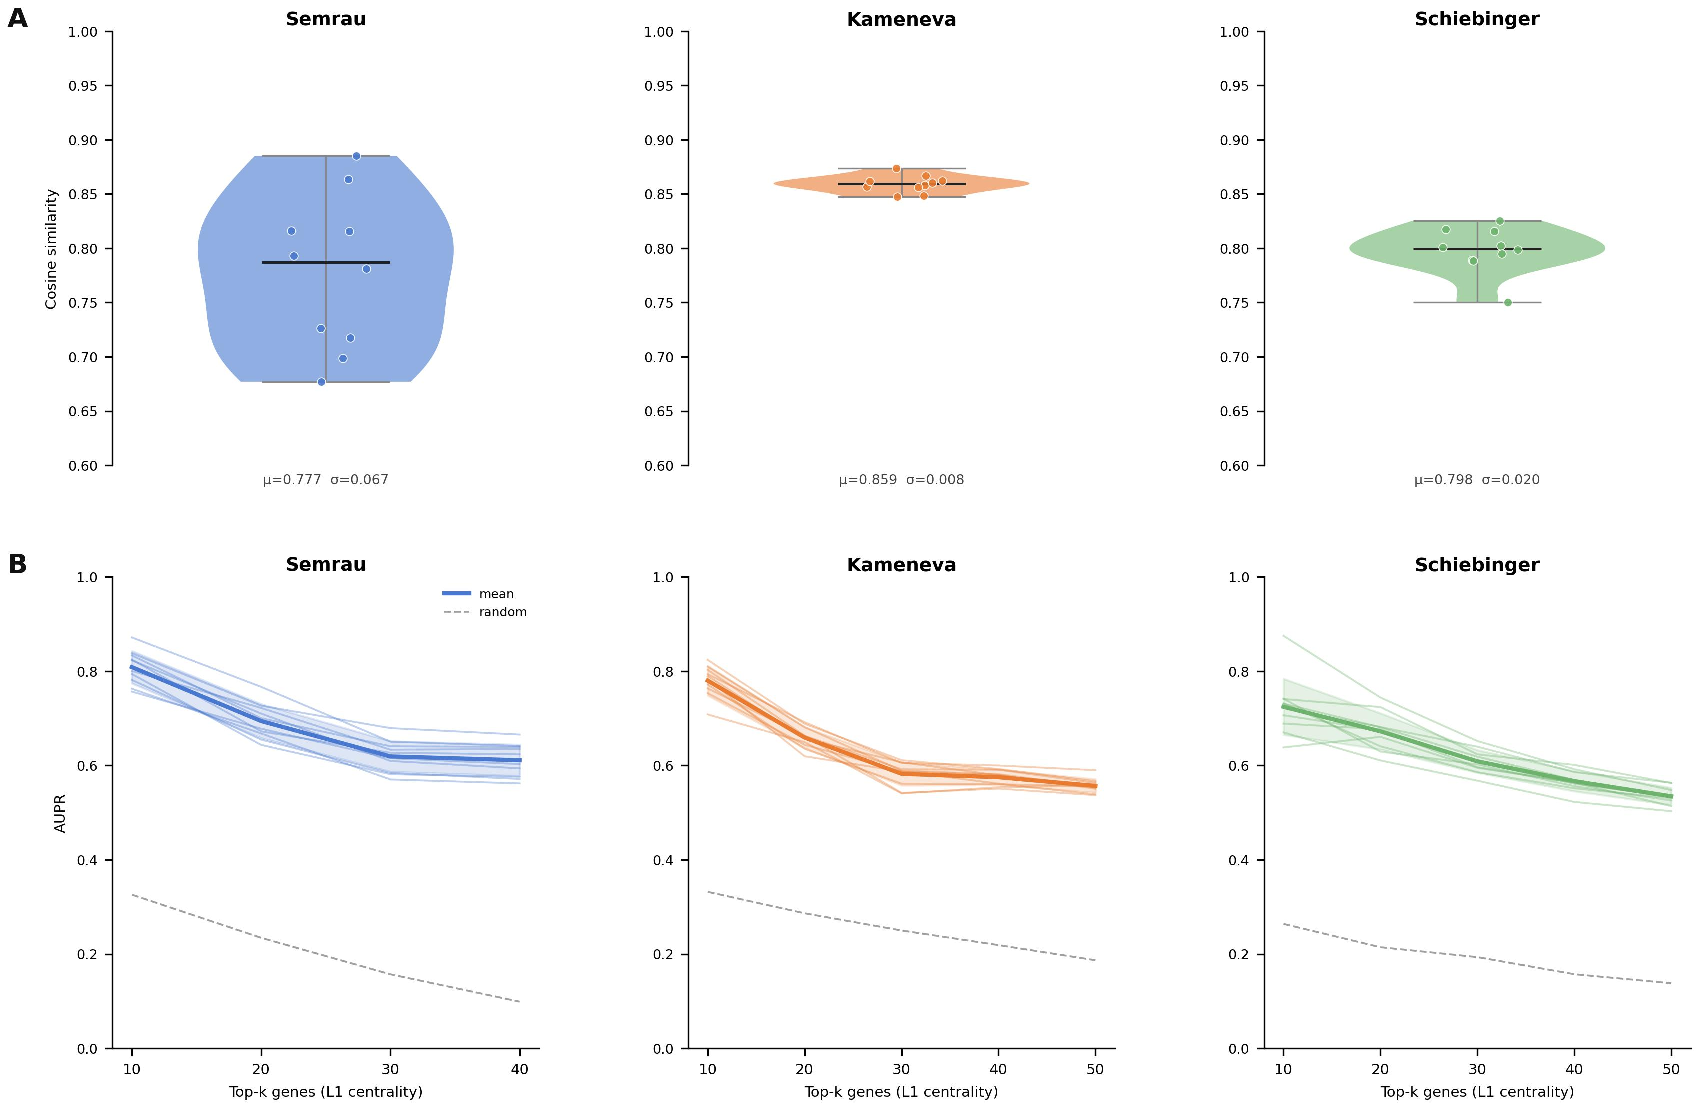
\includegraphics[width=1.0\textwidth]{figureS9.pdf}%
  \caption{%
\firstreview{For each of the three experimental datasets (Semrau, Kameneva, 
Schiebinger), the inference was repeated $N=5$ times independently with 
distinct random initializations. All $\binom{N}{2} = 10$ pairwise comparisons 
between runs are reported symmetrically, without any reference run.
\textbf{(A)}~Pairwise cosine similarity between GRN weight matrices across 
independent runs, displayed as violin plots with individual pairwise values 
overlaid. The mean ($\mu$) and standard deviation ($\sigma$) are reported below 
each violin. 
\textbf{(B)}~Pairwise Area Under the Precision-Recall curve (AUPR) as a 
function of the number of top-ranked genes considered ($k = 10, 20, 30, 40, 
50$), where genes are ranked by their average L1 degree across all runs. For 
each pair of runs $(i, j)$, the GRN from run $i$ is binarized 
(edges with $|w| > 0.5$) and used as ground truth to evaluate the ranking 
provided by run $j$, and vice versa; the two resulting AUPR values are 
averaged. Thin lines represent individual pairwise comparisons; the bold line 
and shaded band show the mean $\pm 1\sigma$ across pairs. The dashed grey line 
indicates the random baseline (network sparsity at each $k$). AUPR values 
substantially exceed the random baseline across all datasets and values of $k$, 
confirming that the inferred GRN topology is reproducible across independent 
runs.}}
  \label{figure_S9}
\end{figure}

\begin{figure}[H]
  \centering
  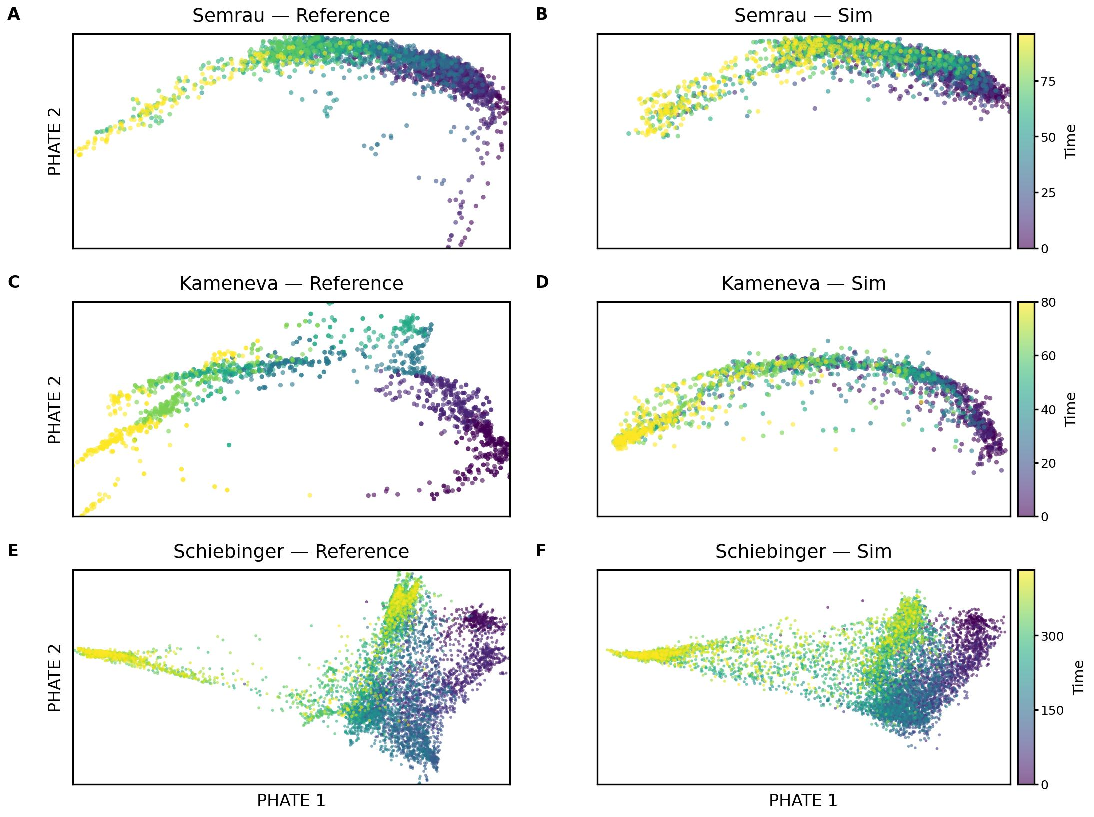
\includegraphics[width=1.0\textwidth]{figureS10.pdf}%
  \caption{%
\firstreview{CardamomOT simulations broadly preserve the global structure and temporal ordering in trajectory-preserving PHATE embeddings. PHATE embeddings of reference (A,C,E) and simulated (B,D,F) RNA data for the 3 differentiation datasets used in the study.}}
  \label{figure_S10}
\end{figure}


\begin{figure}[H]
    \centering
    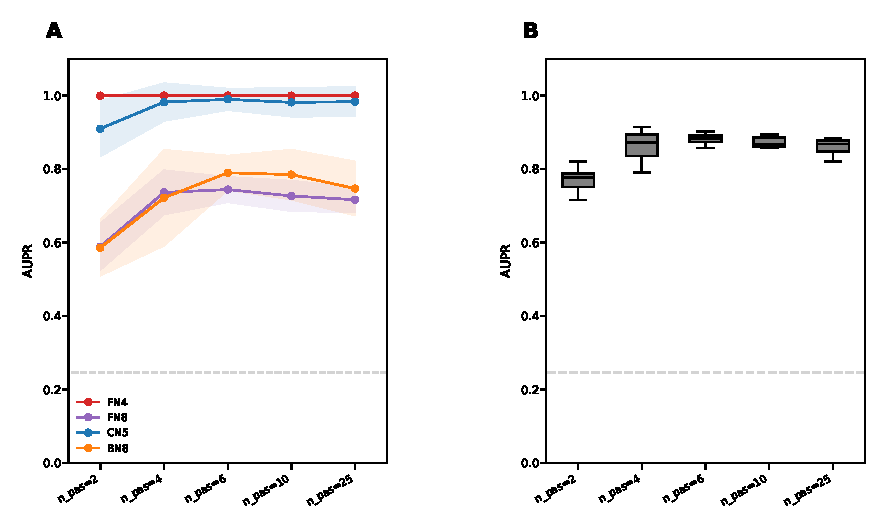
\includegraphics[width=\linewidth]{figureS11.pdf}
    \caption{Sensitivity of GRN inference accuracy to the
switching-time grid resolution $n_{\mathrm{pas}}$. (A) AUPR of CardamomOT across
$n_{\mathrm{pas}}$ levels for each simulated benchmark network (FN4, FN8, CN5, BN8),
shown as mean $\pm$ SD over 10 independent simulations. (B) AUPR for the same runs averaged
across the four benchmark networks. Boxplots show median, interquartile range (box) and
1.5x interquartile range (bars). The dashed gray line indicates the random baseline.}
    \label{figure_S11}
\end{figure}